\documentclass[10pt]{beamer}

% Input setup file with packages and custom commands
% ---------------------------------------------------------------
% Animation: export video frames with
%   ffmpeg -i clip.mp4 -vf fps=12 media/<name>/frame-%d.png
% then uncomment the \animategraphics commands in the frame files.
% NOTE: animation plays only in Adobe Acrobat / pdfpc, NOT macOS Preview.
% ---------------------------------------------------------------
\usepackage{animate}
\usepackage[utf8]{inputenc}
\usepackage{graphicx}
\usepackage {mathtools}
\usepackage{utopia} %font utopia imported
\usetheme{CambridgeUS}
\usecolortheme{dolphin}
\usepackage{algorithm}
\usepackage{algpseudocode}
\usepackage{tikz}
\usetikzlibrary{positioning, arrows.meta, calc, fit, backgrounds, shapes.geometric, decorations.pathreplacing}
\newcommand{\MonthName}{
  \ifcase\month\or January\or February\or March\or April\or May\or June\or July\or August\or September\or October\or November\or December\fi}
% set colors
\definecolor{myNewColorA}{RGB}{150,12,35}
\definecolor{myNewColorB}{RGB}{245,245,245} 
\definecolor{myNewColorC}{RGB}{200,200,200}
\setbeamercolor*{palette primary}{bg=myNewColorC}
\setbeamercolor*{palette secondary}{bg=myNewColorB}
\setbeamercolor*{palette tertiary}{bg=myNewColorA, fg = white}
\setbeamercolor*{titlelike}{fg=myNewColorA}
\setbeamercolor*{title}{bg=myNewColorA, fg = white}
\setbeamercolor*{item}{fg=myNewColorA}
\setbeamercolor*{caption name}{fg=myNewColorA}
\usefonttheme{professionalfonts}
\usepackage[numbers]{natbib}
\usepackage{hyperref}
\usepackage{tabularx}
%------------------------------------------------------------
\titlegraphic{\includegraphics[height=1.5cm]{../../media/uni_logo.jpg}}

\setbeamerfont{title}{size=\large}
\setbeamerfont{subtitle}{size=\small}
\setbeamerfont{author}{size=\small}
\setbeamerfont{date}{size=\small}
\setbeamerfont{institute}{size=\small}

\begin{document}

\title{Autonomous Software Agents: Deliveroo.js}
\author[University of Trento]{%
  Davide Donà\ \ --\ \ \small\texttt{davide.dona-1@studenti.unitn.it}\\
  \small 264467\\
  \and
  Andrea Blushi\ \ --\ \ \small\texttt{andrea.blushi@studenti.unitn.it}\\
  \small 264468
}


\institute[]{ University of Trento}
\date[]{\MonthName\ \number\year}

%The next statement creates the title page.
\frame{\titlepage}
\begin{frame}
\frametitle{Contents}
\tableofcontents
\end{frame}
%------------------------------------------------------------
\section{Introduction}
\label{sec:introduction}
% ----- Our Solution --------------------------------------------
\begin{frame}{Our Solution}
  \begin{itemize}
    \item \textbf{BDI core} - reactive collection, exploration
    \item \textbf{PDDL planner} - crate-clearing
    \item \textbf{LLM layer} - high-level control via structured tools
    \item \textbf{Cooperation} — coordination via peer communication
  \end{itemize}
\end{frame}

\section{BDI Agent}

% ----- Execution Pipeline --------------------------------------
\begin{frame}{Execution Pipeline}
  \begin{columns}
    \column{0.55\textwidth}
      \begin{itemize}
        \item One cycle per \texttt{sensing} socket event
        \item \textbf{Perceive} $\to$ \textbf{Deliberate} $\to$ \textbf{Plan} $\to$ \textbf{Execute}
        \item One action emitted per server clock tick
        \item Re-deliberates after each successful move
      \end{itemize}
    \column{0.42\textwidth}
      % TODO: populate media/pipeline/ with frame images, then uncomment:
      % \animategraphics[autoplay,loop,width=\linewidth]{12}{media/pipeline/frame-}{0}{47}
      \begin{block}{}
        \centering\textit{[agent loop]}
      \end{block}
  \end{columns}
\end{frame}

% ----- Beliefs: Tracker & Memory -------------------------------
\begin{frame}{Beliefs: Tracker \& Memory}
  \begin{itemize}
    \item \textbf{Tracker} — latest observation $\langle v,\, t_{seen} \rangle$ per entity
    \item Confidence decays: $c(t) = e^{-(t - t_{seen})/\tau}$
    \item \textbf{Memory} — bounded temporal history per entity
    \item Observations invalidated when visible-but-absent
  \end{itemize}
\end{frame}

% ----- Beliefs: Map --------------------------------------------
\begin{frame}{Beliefs: Map}
  \begin{itemize}
    \item Static tile layout, transient blocked tiles, traversal penalties
    \item \emph{Sink tiles}: agent can enter but never complete a loop
    \item Modelled as directed walkability graph (conveyors = one-way edges)
    \item Tarjan SCC — only tiles in safe SCCs remain walkable
  \end{itemize}
\end{frame}

% ----- Beliefs: Parcels & Crates -------------------------------
\begin{frame}{Beliefs: Parcels \& Crates}
  \begin{itemize}
    \item Parcel reward decays linearly ($-1$ per server tick) when out of sight
    \item $r(t) = r_0 - \lfloor (t - t_0) / \Delta_t \rfloor$
    \item Parcel removed when $r(t) \leq 0$
    \item Crate positions tracked; invalidated once pushed out of view
  \end{itemize}
\end{frame}

% ----- Desires -------------------------------------------------
\begin{frame}{Desires}
  \begin{itemize}
    \item \textbf{ReachParcel} — navigate to and collect a visible parcel
    \item \textbf{DeliverParcel} — bring carried parcels to delivery tile
    \item \textbf{Explore} — seek unvisited spawn tile when idle
    \item Parcel goals (priority 1) always beat Explore (priority 0)
    \item Intention queue fully rebuilt each deliberation cycle
  \end{itemize}
\end{frame}

% ----- Scoring: Parcels ----------------------------------------
\begin{frame}{Scoring: Parcels}
  \begin{block}{ReachParcel}
    \[ S = \frac{r_p + r_{carried}}{d} \cdot \gamma, \qquad
       \gamma = \min\!\left(1,\, \frac{d_{enemy}}{d}\right) \]
    Race factor $\gamma$ de-prioritises parcels contested by enemies.
  \end{block}
  \begin{block}{DeliverParcel}
    \[ S = \frac{r_{carried}}{d} \]
  \end{block}
\end{frame}

% ----- Scoring: Explore ----------------------------------------
\begin{frame}{Scoring: Explore}
  \begin{itemize}
    \item $w$ — spawn-cluster density (nearby spawn tiles)
    \item $\tau$ — freshness (time since tile was last observed)
    \item $h$ — enemy heat (spatial $+$ temporal Gaussian decay)
    \item $\displaystyle S = \frac{w \cdot \tau}{d \cdot (1 + h)}$
  \end{itemize}
\end{frame}

% ----- Planning: A* --------------------------------------------
\begin{frame}{Planning: A*}
  \begin{columns}
    \column{0.55\textwidth}
      \begin{itemize}
        \item Manhattan distance heuristic (admissible on grid)
        \item Walkability checked dynamically from beliefs
        \item Conveyors: directional movement only
        \item Plan reused while desire type and target unchanged
      \end{itemize}
    \column{0.42\textwidth}
      % TODO: populate media/astar/ with frame images, then uncomment:
      % \animategraphics[autoplay,loop,width=\linewidth]{12}{media/astar/frame-}{0}{47}
      \begin{block}{}
        \centering\textit{[pathfinding]}
      \end{block}
  \end{columns}
\end{frame}

% ----- Collision Handling --------------------------------------
\begin{frame}{Collision Handling}
  \begin{columns}
    \column{0.55\textwidth}
      Next tile occupied? Three-stage escalation:
      \begin{enumerate}
        \item \textbf{Detour} — replan with tile as wall (within cost threshold)
        \item \textbf{Wait} — random pause duration
        \item \textbf{Block \& replan} — temporary TTL block, full replan
      \end{enumerate}
    \column{0.42\textwidth}
      % TODO: populate media/collision/ with frame images, then uncomment:
      % \animategraphics[autoplay,loop,width=\linewidth]{12}{media/collision/frame-}{0}{47}
      \begin{block}{}
        \centering\textit{[collision resolution]}
      \end{block}
  \end{columns}
\end{frame}

\section{PDDL Crate Navigation}
% ----- When A* Fails ---------------------------------------------
\begin{frame}{When A* Fails}
    \begin{itemize}
        \item A* fails: no path that avoids crates
        \item Second A* ignoring crates finds a ``ghost'' path
        \item Crates intersecting that path are part of the ``PDDL`` problem instance
    \end{itemize}
\end{frame}

% ----- PDDL  -------------------------------------------
\begin{frame}{PDDL}
  \begin{columns}
    \column{0.55\textwidth}
      \begin{itemize}
        \item Cluster detected $\to$ PDDL problem built from current beliefs
        \item Solver finds \texttt{move} + \texttt{push} sequence to reach goal
        \item Result translated back to agent's action plan
      \end{itemize}
    \column{0.43\textwidth}
      %#TODO: uncomment this for video demo
      %\animategraphics[autoplay,loop,width=\linewidth]{12}{../../media/PDDL/frame-}{1}{256}
      \begin{block}{}
        \centering\textit{[PDDL demo]}
      \end{block}
  \end{columns}
\end{frame}

% ----- Performance Bottlenecks ----------------------------------
\begin{frame}{Performance Bottlenecks}
  \begin{itemize}
    \item \textbf{Real-Time Constraints:} The initial PDDL solver integration was too slow to meet the game's strict timing demands.
    \item \textbf{Identified Issues \& Fixes:}
    \begin{itemize}
      \item \emph{API Overhead:} Remote solver calls introduced heavy latency. \textbf{Fix:} Migrated to a local solver instance.
      \item \emph{Redundant Computation:} Identical crate configurations were being solved repeatedly, but implementing a standard cache was non-trivial.
    \end{itemize}
    \item \textbf{The Pivot:} Rather than brute-forcing a complex caching mechanism, we restated the problem to naturally maximize cache hits.
  \end{itemize}
\end{frame}

% ----- Smart Fix -----------------------------------------------
\begin{frame}{Optimization: Problem Restatement}
  \begin{block}{Three-Phase Journey Segmentation}
    \begin{enumerate}
      \item \textbf{Approach:} A* pathfinding from the current position to the cluster \emph{entry}.
      \item \textbf{Manipulation:} PDDL execution solely through the crate cluster (entry $\to$ exit).
      \item \textbf{Completion:} A* pathfinding from the cluster \emph{exit} to the final goal.
    \end{enumerate}
  \end{block}
\end{frame}

% ----- Smart Fix (Result) --------------------------------------
\begin{frame}{Optimization: Problem Restatement}
  \begin{columns}
    \column{0.4\textwidth}
      \begin{itemize}
        \item \textbf{The Result:} The PDDL problem is now strictly anchored to the cluster entry tile rather than absolute map coordinates.
        \item \textbf{Simplified Cache Key:} $\langle \text{entry},\, \text{exit},\, \{\text{crate positions}\} \rangle$.
      \end{itemize}
    \column{0.55\textwidth}
        \centering
        \resizebox{\linewidth}{!}{% Three-segment path decomposition (A* -> PDDL -> A*).
% Requires tikz libraries: arrows.meta, backgrounds, shapes.geometric.
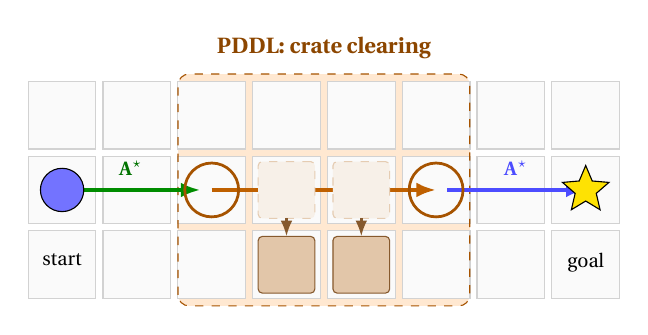
\begin{tikzpicture}[
  x=0.95cm, y=0.95cm,
  tile/.style={draw=gray!35, fill=gray!4, minimum size=0.86cm, inner sep=0},
  crate/.style={draw=brown!70!black, fill=brown!45, minimum size=0.72cm, inner sep=0, rounded corners=1.5pt},
  ghost/.style={draw=brown!40, fill=brown!12, minimum size=0.72cm, inner sep=0, rounded corners=1.5pt, dashed},
  agent/.style={draw=black, fill=blue!55, circle, minimum size=0.55cm, inner sep=0},
  goal/.style={star, star points=5, star point ratio=2.2, draw=black, fill=yellow!85!orange, minimum size=0.62cm, inner sep=0},
  push/.style={-{Latex[length=2mm]}, brown!70!black, line width=0.9pt},
]
  % --- tile grid: 8 cols (0..7) x 3 rows (0..2) ---
  \foreach \x in {0,...,7}{
    \foreach \y in {0,1,2}{ \node[tile] at (\x,\y) {}; }
  }

  % --- PDDL cluster region highlight ---
  \begin{scope}[on background layer]
    \fill[orange!18, rounded corners=4pt] (1.55,-0.55) rectangle (5.45,2.55);
  \end{scope}
  \draw[orange!65!black, dashed, rounded corners=4pt] (1.55,-0.55) rectangle (5.45,2.55);
  \node[orange!55!black, font=\footnotesize\bfseries] at (3.5,2.9) {PDDL: crate clearing};

  % --- A* segments (green approach, blue exit) ---
  \draw[green!55!black, line width=1.7pt, -{Latex[length=2.5mm]}] (0,1) -- (1.85,1)
    node[midway, above=1pt, font=\scriptsize\bfseries, green!45!black] {A$^\star$};
  \draw[blue!70, line width=1.7pt, -{Latex[length=2.5mm]}] (5.15,1) -- (7,1)
    node[midway, above=1pt, font=\scriptsize\bfseries, blue!70] {A$^\star$};

  % --- PDDL traversal arrow through the cleared corridor ---
  \draw[orange!75!black, line width=1.5pt, -{Latex[length=2.5mm]}] (2,1) -- (5,1);

  % --- crates: ghost in original blocking spot, solid after push ---
  \node[ghost] at (3,1) {};
  \node[ghost] at (4,1) {};
  \node[crate] at (3,0) {};
  \node[crate] at (4,0) {};
  \draw[push] (3,0.62) -- (3,0.38);
  \draw[push] (4,0.62) -- (4,0.38);

  % --- agent, goal, entry/exit markers ---
  \node[agent] at (0,1) {};
  \node[goal]  at (7,1) {};
  \draw[orange!65!black, line width=1pt] (2,1) circle (0.36);
  \draw[orange!65!black, line width=1pt] (5,1) circle (0.36);
  \node[font=\scriptsize, below=0.30cm] at (0,0.6) {start};
  \node[font=\scriptsize, below=0.30cm] at (7,0.6) {goal};
\end{tikzpicture}
}
  \end{columns}
\end{frame}

\section{LLM Agent Layer}

% ----- LLM Layer Overview --------------------------------------
\begin{frame}{LLM Layer Overview}
  \begin{itemize}
    \item Thin wrapper around the BDI core
    \item Listens and interprets mission-controller chat messages
    \item Modifies the BDI behaviour accordingly
    \item Four command categories: \textbf{goal injection}, \textbf{rules}, \textbf{coordination} and \textbf{cooperation}
  \end{itemize}
\end{frame}

% ----- Goal Injection ------------------------------------------
\begin{frame}{Goal Injection}
  \begin{exampleblock}{Trigger Examples}
    \begin{itemize}
      \item \textit{``Move to coordinate (4,7) and you get +10pts''}
      \item \textit{``Drop a package in the leftmost tile to get 5pt''}
    \end{itemize}
  \end{exampleblock}
  
  \vspace{1em}
  
  \begin{itemize}
    \item LLM can inject new goals into the BDI agent (e.g. \texttt{go-to}, \texttt{deliver-at})
    \item Compete with existing BDI desires; may be accepted or rejected
    \item Persist and re-evaluated until executed or TTL expires
    \item \textbf{Peer-injection}: the LLM applies the command locally, then repackages it and broadcasts it
  \end{itemize}
\end{frame}

% ----- Goal Injection (diagram) --------------------------------
\begin{frame}{Goal Injection: Local + Peer Broadcast}
  \centering
  \resizebox{0.92\textwidth}{!}{% LLM goal injection: local inject + peer broadcast, located at the BDI merge stage.
% Requires tikz libraries: positioning, arrows.meta, fit, backgrounds.
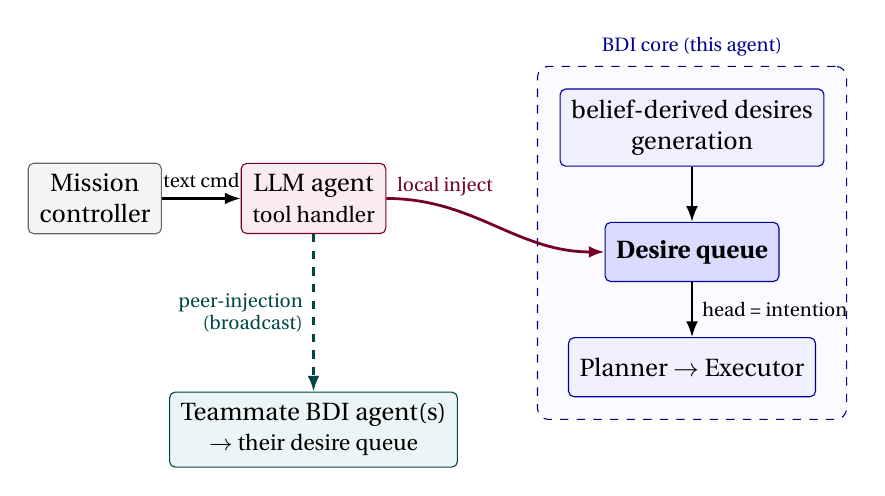
\begin{tikzpicture}[
  font=\small,
  node distance=6mm,
  box/.style={draw=black!60, rounded corners=2pt, align=center, inner sep=4pt,
              minimum height=0.75cm},
  llm/.style={box, draw=purple!60!black, fill=purple!8},
  core/.style={box, draw=blue!60!black, fill=blue!6},
  merge/.style={box, draw=blue!60!black, fill=blue!14, font=\small\bfseries},
  peer/.style={box, draw=teal!55!black, fill=teal!8},
  flow/.style={-{Latex[length=2mm]}, line width=0.8pt},
  inject/.style={-{Latex[length=2mm]}, line width=1pt, purple!60!black},
  bcast/.style={-{Latex[length=2mm]}, line width=1pt, teal!55!black, dashed},
]
  % --- mission controller + LLM agent ---
  \node[box, fill=gray!8] (mc) {Mission\\controller};
  \node[llm, right=10mm of mc] (tool) {LLM agent\\\footnotesize tool handler};
  \draw[flow] (mc) -- (tool) node[midway, above, font=\scriptsize] {text cmd};

  % --- this agent's BDI core (compact: only the injection point) ---
  \node[core, right=22mm of tool, yshift=9mm] (bel)
    {belief-derived desires\\ generation};
  \node[merge, below=7mm of bel] (queue) {Desire queue};
  \node[core, below=7mm of queue] (exec) {Planner $\rightarrow$ Executor};
  \draw[flow] (bel) -- (queue);
  \draw[flow] (queue) -- node[right, font=\scriptsize] {head = intention} (exec);

  \begin{scope}[on background layer]
    \node[draw=blue!55!black, dashed, rounded corners=4pt, fill=blue!2,
          fit=(bel)(queue)(exec), inner sep=8pt,
          label={[blue!55!black,font=\scriptsize]above:BDI core (this agent)}] (corebox) {};
  \end{scope}

  % --- teammates ---
  \node[peer, below=20mm of tool] (peeragents)
    {Teammate BDI agent(s)\\\footnotesize $\rightarrow$ their desire queue};

  % --- injections ---
  \draw[inject] (tool.east) to[out=0, in=180]
    node[above, font=\scriptsize, pos=0.25] {local inject} (queue.west);
  \draw[bcast] (tool.south) --
    node[left, font=\scriptsize, align=right] {peer-injection\\(broadcast)} (peeragents.north);
\end{tikzpicture}
}
\end{frame}

% ----- Rule Injection ------------------------------------------
\begin{frame}{Rule Injection}
  \begin{exampleblock}{Trigger Examples}
    \begin{itemize}
      \item \textit{``Deliver stacks of exactly 3 parcels at a time to double the reward''}
      \item \textit{``Every time you deliver in (x1,y1) you get 0 pts''}
    \end{itemize}
  \end{exampleblock}
  
  \vspace{1em}
  
  \begin{itemize}
    \item \texttt{RuleStore}: Defines a condition, multiplier ($m$), and offset ($a$)
    \item \textbf{Effect}: Dynamically scales and shifts the BDI score for any desire matching the condition
    \item \textbf{Special case}: The \textbf{Stack rule} automatically elevates \textbf{Explore} to priority~1
  \end{itemize}
\end{frame}

% ----- Coordination: Position Sharing --------------------------------------
\begin{frame}{Coordination: Position Sharing}
  \begin{itemize}
    \item \textbf{Beacons}: each agent broadcasts position at fixed interval
    \item Ensures up-to-date peer positions beyond sensing radius
    \item Needed for coordination when agents are outside each other's sensing radius
  \end{itemize}
\end{frame}

% ----- Coordination: 2-Phase Commit -----------------------------------
\begin{frame}{Coordination: 2-Phase Commit}
  \begin{exampleblock}{Trigger Example}
    \begin{itemize}
      \item \textit{``Move both agents to the neighborhood of position (x,y) within a maximum distance of 3, and have them wait for each other. You will receive 500pts.''}
    \end{itemize}
  \end{exampleblock}
  
  \vspace{1em}
  
  Used for complex coordination tasks (commit together or not at all):
  \begin{itemize}
    \item \textbf{Phase 1 - Propose}: proposer broadcasts candidate hold tiles; each agent scores them
    \item \textbf{Vote}: \emph{accept} if the hold outweighs current desires; \emph{reject} if current desires are better
    \item \textbf{Phase 2 - Decide}: unanimous accept $\to$ commit (all inject); any miss or reject $\to$ abort
  \end{itemize}
\end{frame}

% ----- Coordination: 2-Phase Commit (diagram) ------------------
\begin{frame}{Coordination: 2-Phase Commit}
  \centering
  \resizebox{0.95\textwidth}{!}{% Two-phase commit sequence diagram for synchronized holds.
% Requires tikz libraries: arrows.meta, calc, decorations.pathreplacing.
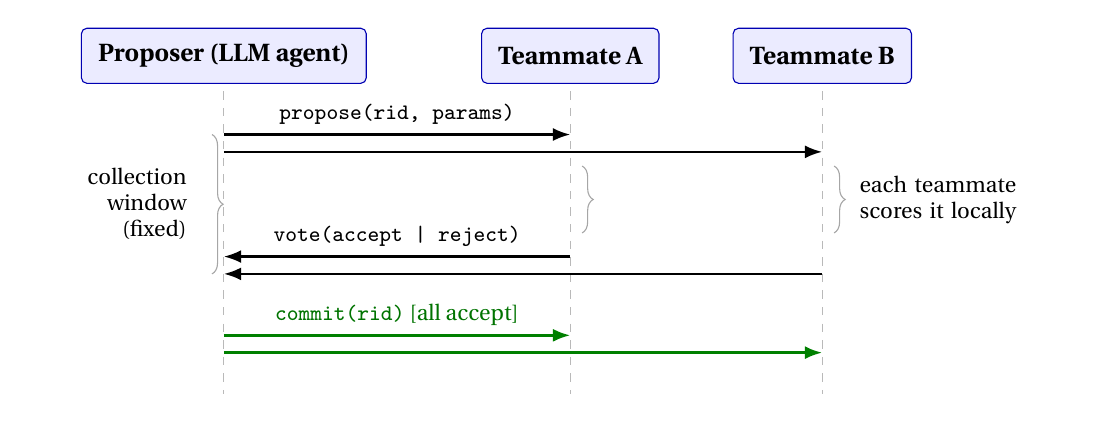
\begin{tikzpicture}[
  font=\small,
  head/.style={draw=blue!70!black, fill=blue!8, rounded corners=2pt,
               minimum height=0.7cm, inner xsep=6pt, font=\small\bfseries},
  msg/.style={-{Latex[length=2.2mm]}, line width=0.9pt},
  commit/.style={-{Latex[length=2.2mm]}, line width=1pt, green!50!black},
  evalbrace/.style={decorate, decoration={brace, amplitude=4pt}, gray!70},
]
  % --- lifeline x positions ---
  \def\P{0} \def\A{4.4} \def\B{7.6}
  \def\Bot{-4.3}

  % --- heads ---
  \node[head] (hP) at (\P,0) {Proposer (LLM agent)};
  \node[head] (hA) at (\A,0) {Teammate A};
  \node[head] (hB) at (\B,0) {Teammate B};

  % --- lifelines ---
  \foreach \x in {\P,\A,\B}{ \draw[gray!55, dashed] (\x,-0.45) -- (\x,\Bot); }

  % --- Phase 1: propose (broadcast) ---
  \draw[msg] (\P,-1.0) -- (\A,-1.0);
  \draw[msg] (\P,-1.22) -- (\B,-1.22);
  \node[above, font=\footnotesize] at ($(\P,-1.0)!0.5!(\A,-1.0)$) {\texttt{propose(rid, params)}};

  % --- each teammate evaluates the proposal locally (brace, like the collection window) ---
  \draw[evalbrace] (\A+0.15,-1.4) -- (\A+0.15,-2.25);
  \draw[evalbrace] (\B+0.15,-1.4) -- (\B+0.15,-2.25);
  \node[anchor=west, font=\footnotesize, text width=2.5cm, align=left]
    at (\B+0.35,-1.83) {each teammate scores it locally};

  % --- votes ---
  \draw[msg] (\A,-2.55) -- (\P,-2.55);
  \draw[msg] (\B,-2.77) -- (\P,-2.77);
  \node[above, font=\footnotesize] at ($(\A,-2.55)!0.5!(\P,-2.55)$) {\texttt{vote(accept | reject)}};

  % --- collection window on proposer ---
  \draw[evalbrace] (\P-0.15,-1.0) -- (\P-0.15,-2.77);
  \node[anchor=east, font=\footnotesize, text width=1.9cm, align=right]
    at (\P-0.35,-1.88) {collection window (fixed)};

  % --- Phase 2: commit (if unanimous accept) ---
  \draw[commit] (\P,-3.55) -- (\A,-3.55);
  \draw[commit] (\P,-3.77) -- (\B,-3.77);
  \node[above, font=\footnotesize, green!45!black]
    at ($(\P,-3.55)!0.5!(\A,-3.55)$) {\texttt{commit(rid)} \footnotesize[all accept]};
\end{tikzpicture}
}
\end{frame}

% ----- Cooperation: Motivation -------------------------
\begin{frame}{Cooperation: Motivation}
  \begin{exampleblock}{Origin: Admin Directive}
    \textit{``If a parcel is initially picked up by one agent and later delivered by the other agent, you will receive a 200 points bonus.''}
  \end{exampleblock}

  \vspace{1em}
  \begin{itemize}
    \item A one-shot \emph{check-and-coordinate} is insufficient: requires dynamic pickups, meeting tile computations, and joint commitments.
    \item[$\Rightarrow$] Solution: Dedicated \textbf{roles} with specific behaviours, agreed upon via a \textbf{2-phase commit} (2PC).
    \item Generalised into a reusable framework of \textbf{strategies} and \textbf{roles}.
  \end{itemize}
\end{frame}

% ----- Cooperation: Generalisation -------------------------
\begin{frame}{Cooperation: Generalisation}
  \begin{itemize}
    \item A \textbf{cooperation round} opens every $\Delta t$ seconds (or immediately upon a mission directive).
    \item Agents request teammates' beliefs to build a \textbf{shared compact context}:
  \end{itemize}
  
  \begin{block}{Context State}
      \begin{itemize}
        \item \textbf{Roster}: Positions, payloads, sensed enemies.
        \item \textbf{Map Geometry}: Spawn/delivery clusters, separation, corridor flags.
        \item \textbf{Performance}: Average score/round per strategy (sliding window).
      \end{itemize}
  \end{block}

  \begin{itemize}
    \item[$\Rightarrow$] The \textbf{LLM} evaluates this context to select the optimal shared strategy for the team.
  \end{itemize}
\end{frame}

% ----- Cooperation: Strategies ---------------------------------
\begin{frame}{Cooperation: Strategies}
  \begin{itemize}
    \item \texttt{ZONAL\_RELAY}: One agent sweeps the spawn region and drops at a fixed midpoint; the companion ferries parcels to delivery.
    \item \texttt{OPPORTUNISTIC}: Agents forage independently and hand off parcels dynamically upon pickup.
    \item \texttt{NONE}: Fully autonomous baseline (no cooperation).
  \end{itemize}
\end{frame}

% ----- Cooperation: Roles --------------------------------------
\begin{frame}{Cooperation: Roles}
  \begin{itemize}
    \item Each strategy assigns every agent a specific \textbf{role}.
    \item Standard BDI desire generation is \emph{blocked}.
    \item A role-specific \textbf{FSM} generates desires dynamically based on the shared context and internal state.
    \item Meeting points and positioning are computed \emph{deterministically} from the map's geometry.
  \end{itemize}
\end{frame}

% ----- Cooperation: Handpass -----------------------------------
\begin{frame}{Cooperation: Handpass}
  \begin{columns}
    \column{0.60\textwidth}
      Both strategies culminate in a \textbf{handpass}:
      \vspace{0.5em}
      \begin{itemize}
        \item \texttt{ZONAL\_RELAY}:\\ The exchange loops indefinitely at the designated midpoint.
        \vspace{0.5em}
        \item \texttt{OPPORTUNISTIC}:\\ The agent acquiring a parcel proposes a handpass via 2PC.
      \end{itemize}
      
    \column{0.38\textwidth}
      %#TODO: uncomment this for video demo
      %\animategraphics[autoplay,loop,width=\linewidth]{12}{../../media/cooperation/frame-}{1}{196}
      \begin{block}{}
        \centering\textit{[Collaboration demo]}
      \end{block}
  \end{columns}
\end{frame}


\section*{References}  
\begin{frame}
\nocite{*}
\bibliographystyle{ieeetr} 
\small{\bibliography{references}}
\end{frame}
\end{document}